\section{Dữ liệu và xây dựng benchmark}\label{sec:data}

\subsection{Corpus và chạy lại trong môi trường cách ly}\label{sec:replay}
Chúng tôi dùng các bài nộp gốc của C-Pack-IPAs bản phát hành~26 \citep{orvalho2024cpack}: {{n_submissions}} chương trình C90 của {{n_students}} sinh viên ẩn danh cho 25 bài tập thuộc ba buổi thực hành, với {{n_tests}} test đầu vào/đầu ra. Log lịch sử ghi verdict từng test nhưng thường không lưu output của test đạt, và {{n_not_run_cells}} ô test chưa từng được chạy hoặc không được ghi log. Để có đủ bằng chứng thực thi, chúng tôi chạy lại mọi chương trình không rỗng trong một container chỉ dùng cho nghiên cứu: không mạng, hệ thống tệp gốc chỉ đọc, bỏ mọi quyền Linux trừ các quyền cần để chuyển sang một người dùng không đặc quyền riêng cho mỗi lượt chạy, với giới hạn {{cpu_limit}}~giây CPU, {{wall_limit}}~giây thời gian thực và 512~MiB bộ nhớ cho mỗi test. Chương trình được biên dịch bằng \texttt{gcc} {{gcc_version}} với cờ của khóa học (\texttt{-ansi -pedantic -Wall -Wextra}); vì khóa học còn dùng \texttt{-Werror}, chúng tôi ghi lại việc biên dịch có sạch cảnh báo hay không thay vì loại chương trình. Container chỉ trả về các byte output thô; oracle nằm ở máy chủ, nơi quyết định mọi verdict.

Lần chạy lại khớp {{audit_cells_pct}}\% trong {{audit_cells}} verdict test lịch sử theo chính sách khớp chính xác và mã thoát 0 (được chọn trên partition huấn luyện trong bốn chính sách so sánh; \cref{tab:audit}), tái tạo byte-đúng-byte output đã ghi của {{audit_stdout_pct}}\% các câu trả lời sai lịch sử, và khớp kết quả biên dịch lịch sử theo ngữ nghĩa \texttt{-Werror} với {{audit_compile_pct}}\% chương trình. Một lần chạy lại độc lập thứ hai từ commit sạch khớp {{repro_cells_pct}}\% ô test; {{n_unstable}} chương trình có kết quả khác nhau giữa hai lần (nhiều khả năng do hành vi không xác định) bị loại khỏi mọi item (sửa đổi~A5).

\begin{table}[t]
\centering
\caption{Tỷ lệ khớp (\%) giữa lần chạy lại cách ly và verdict lịch sử từng test theo bốn chính sách so sánh output. Chính sách được chọn trên partition huấn luyện trước khi có bất kỳ nhãn cơ chế nào.}\label{tab:audit}
\small
\begin{tabular}{lrrr}
\toprule
Chính sách so sánh & Huấn luyện & Kiểm định & Kiểm tra \\
\midrule
{{table_audit}}
\bottomrule
\end{tabular}
\end{table}

\subsection{Chia dữ liệu}
Bài nộp được chia trước khi có bất kỳ nhãn nào thành các partition huấn luyện, kiểm định và kiểm tra (70/15/15\% số thành phần liên thông), sao cho mọi bài của một sinh viên, xuyên năm và xuyên bài tập, cùng mọi mã nguồn trùng byte đều nằm trong một partition. Mọi item suy ra đều thừa kế partition của bài nộp gốc.

\subsection{Nhãn dựa trên bản sửa}\label{sec:real}
Với mỗi bài nộp sai (ít nhất một test không đạt), chúng tôi tìm lần nộp kế tiếp của cùng sinh viên, cùng bài tập, cùng năm mà đạt mọi test. Với mỗi sự kiện sửa như vậy, chúng tôi giữ lần nộp sai cuối cùng trước nó (sửa đổi~A2), được {{n_pairs}} cặp sai--đã sửa. \Cref{alg:label} tóm tắt cách một cặp trở thành nhãn. Khác biệt theo dòng giữa hai chương trình, bỏ qua thụt lề, được chia thành các hunk. Delta debugging theo hunk \citep{zeller2002ddmin} tìm một tập con 1-tối thiểu các hunk mà khi áp vào bài sai thì bài đạt mọi test; mọi ứng viên đều được chạy trong runner cách ly (ngân sách {{ddmin_budget}} lần thử mỗi cặp). Cả hai đầu mút được kiểm lại trong cùng runner trước khi tìm.

Thay đổi tối thiểu đã kiểm chứng được một bộ phân loại tất định xếp vào một trong mười hai loại mức chương trình (\cref{tab:taxonomy}); bộ phân loại làm việc trên từng hunk đã kiểm chứng: câu lệnh được chèn hoặc xóa nguyên vẹn được nhận ra sau khi trượt đoạn token về biên câu lệnh, các dòng giống hệt bị xóa ở chỗ này và chèn ở chỗ khác là thay đổi vị trí, còn mọi token thay đổi khác được quy về ngữ cảnh cú pháp gần nhất có vai trò xác định (đầu vòng lặp, điều kiện rẽ nhánh, giá trị khởi tạo, định dạng in, \dots). Một cặp chỉ nhận nhãn đơn cơ chế khi bản sửa tối thiểu thuộc đúng một loại khác \textsc{Other}; bản sửa trải nhiều loại được giữ là \textsc{Multi} và không vào tập nhãn chuẩn chính. Bài sửa, bản vá và nhãn không bao giờ được dùng làm đặc trưng. \Cref{fig:flow}A ghi lại mọi bước loại trừ.

\begin{algorithm}[t]
\caption{Gán nhãn từ bản sửa cho một sự kiện sửa}\label{alg:label}
\begin{algorithmic}[1]
\Require bài sai $f$; lần nộp kế tiếp $p$ của cùng sinh viên đạt mọi test của bộ test $T$
\State chạy $f$ và $p$ trên $T$ trong runner cách ly; dừng nếu $f$ không trượt test nào hoặc $p$ không đạt hết \Comment{hai đầu mút}
\State $H \gets$ các hunk dòng của $\mathrm{diff}(f, p)$, bỏ qua thụt lề
\State $H^\star \gets \mathrm{ddmin}(H)$, trong đó tập con $S \subseteq H$ thành công khi $f$ vá bằng $S$ biên dịch được và đạt mọi test của $T$
\State $C \gets \{\text{loại}(h) : h \in H^\star\}$ \Comment{vai trò cú pháp của từng token thay đổi}
\If{$C = \{c\}$ và $c \neq \textsc{Other}$}
  \State \Return nhãn $c$
\Else
  \State \Return \textsc{Multi} hoặc \textsc{Other} (không vào nhãn chuẩn)
\EndIf
\end{algorithmic}
\end{algorithm}

\subsection{Tiêm cơ chế có kiểm soát}\label{sec:injected}
Bản sửa thật có giá trị sinh thái nhưng nhiễu, mất cân bằng và phụ thuộc điều sinh viên tình cờ làm. Vì vậy chúng tôi xây thêm một benchmark kiểm soát. Từ các chương trình đã đạt và sạch cảnh báo (tối đa {{max_sources}} bài mỗi bài tập, mỗi sinh viên và năm một bài), chúng tôi sinh mutant một thay đổi bằng các toán tử khớp với cùng taxonomy: độ chặt của phép so sánh trong vòng lặp hoặc điều kiện, phép nối logic, điểm bắt đầu vòng lặp, giá trị khởi tạo hằng, toán tử số học, bỏ ép kiểu thực hoặc hằng thực, độ chính xác của printf, bỏ ký tự xuống dòng cuối, chữ hoa/thường của văn bản in, xóa câu lệnh, lặp câu lệnh, và chuyển câu lệnh vào trong vòng lặp. Mỗi loại và mỗi bài gốc được đột biến ở một vị trí ngẫu nhiên với seed cố định. Mutant chỉ được giữ nếu biên dịch sạch cảnh báo và trượt ít nhất một test, tức là có thể đã là một bài nộp sai thật của khóa học (\cref{fig:flow}B). Một unit test kiểm tra rằng bộ phân loại ở \cref{sec:real} xếp phép sửa ngược của mọi toán tử vào đúng loại của toán tử, nên hai bộ nhãn dùng chung một định nghĩa.

\begin{figure}[tbp]
\centering
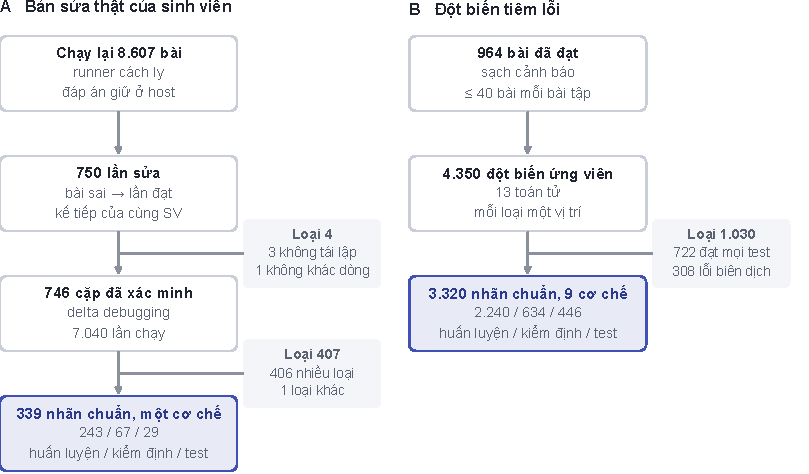
\includegraphics[width=\textwidth]{figures/fig3_flow_vi.pdf}
\caption{Quá trình xây hai benchmark. (A) Bản sửa thật của sinh viên: {{real_one_minimal}} trong {{real_ok}} cặp đã kiểm chứng đạt tập con 1-tối thiểu trong ngân sách thử; ba cặp còn lại đều trải nhiều loại. (B) Mutant tiêm lỗi: ứng viên vẫn đạt mọi test (tương đương trên bộ test) hoặc biên dịch không sạch bị loại. Kích thước partition theo thứ tự huấn luyện / kiểm định / kiểm tra.}\label{fig:flow}
\end{figure}

\begin{table}[t]
\centering
\caption{Taxonomy cơ chế mức chương trình. Một loại mô tả điều mà bản sửa tối thiểu đã kiểm chứng (hoặc thay đổi được tiêm) thay đổi; cột phải là giả thuyết quan niệm sai để giảng viên kiểm tra, không phải chẩn đoán.}\label{tab:taxonomy}
\small
\begin{tabular}{p{2.9cm}p{4.9cm}p{4.6cm}}
\toprule
Loại & Thay đổi tối thiểu sửa\dots & Giả thuyết cần kiểm tra \\
\midrule
Biên vòng lặp & điều kiện, điểm bắt đầu hoặc bước nhảy của vòng lặp & lệch một, chỉ số từ 0 hay 1 \\
Điều kiện rẽ nhánh & điều kiện hoặc cấu trúc if/switch/else & biên so sánh, \texttt{\&\&} và \texttt{||} \\
Khởi tạo & giá trị khởi tạo khi khai báo hoặc gán hằng ngoài vòng lặp & khởi tạo biến tích lũy, giá trị lớn nhất \\
Biểu thức tính & toán tử, toán hạng trong phép gán, return, biểu thức được in & công thức, độ ưu tiên toán tử \\
Kiểu số & kiểu, ép kiểu, hằng thực, hàm toán học & chia nguyên \\
Định dạng in & đặc tả chuyển đổi của printf & độ chính xác, độ rộng \\
Văn bản in & chữ trong output hoặc lệnh chỉ in hằng & đọc đặc tả output \\
Đọc dữ liệu & lời gọi scanf/getchar & định dạng đầu vào, EOF \\
Vị trí câu lệnh & câu lệnh hoặc dấu ngoặc bị di chuyển & phạm vi khối, đặt lại biến trong vòng lặp \\
Thiếu bước & chèn nguyên câu lệnh & thiếu cập nhật hoặc trường hợp \\
Thừa bước & xóa nguyên câu lệnh & cập nhật hai lần, in gỡ lỗi \\
Luồng điều khiển & break/continue/return & thoát sớm \\
\bottomrule
\end{tabular}
\end{table}

\section{Phương pháp}\label{sec:methods}

\subsection{Biểu diễn đối tượng--thuộc tính--giá trị}\label{sec:reps}
Mỗi chương trình sai (đối tượng) được mô tả bằng các thuộc tính phân loại chỉ tính từ chính chương trình và các lượt chạy lại của nó. Gọi $T$ là tập test của một bài tập, $y_t$ là output đúng của test $t$, và $\hat y_t(o)$ là output của chương trình $o$. OAV kết quả test của cách phát biểu kinh điển là
\begin{equation}
x^{\mathrm{out}}(o) = \bigl(r_t(o)\bigr)_{t \in T}, \qquad r_t(o) \in \{\text{đạt}, \text{sai}, \text{lỗi chạy}, \text{quá thời gian}\}.
\end{equation}
\emph{OAV độ lệch} thêm, với mỗi test, $K = 9$ mô tả không cần nhãn $d_k\bigl(\hat y_t(o), y_t\bigr)$ về cách output lệch khỏi đáp án---trạng thái chạy, số dòng, ký tự xuống dòng cuối, chỉ khác khoảng trắng, quan hệ giữa các số tương ứng (lệch một, bị cắt phần thập phân, độ chính xác, dấu, bằng không, tỷ lệ, chỉ khác cách viết), quan hệ giữa các từ (chỉ khác hoa/thường, lỗi chính tả, thiếu hoặc thừa từ), vị trí dòng khác đầu tiên, quan hệ tiền tố và việc trùng đáp án của test khác---cùng giá trị phổ biến nhất của chúng trên các test sai,
\begin{equation}
\bar d_k(o) = \operatorname{mode}\bigl\{ d_k\bigl(\hat y_t(o), y_t\bigr) : r_t(o) \neq \text{đạt} \bigr\},
\end{equation}
và tỷ lệ test sai. Khối gộp $\bar d(o)$ không phụ thuộc bài tập, nên so sánh được giữa các bài; \cref{fig:example} cho thấy giá trị của nó với ba chương trình có cùng một chữ ký test. Từ vựng được khớp, không dùng nhãn, trên các bài sai thuộc partition huấn luyện của cùng bài tập; giá trị chưa gặp khi huấn luyện được ánh xạ thành \emph{chưa biết}. Chúng tôi so sánh tám biểu diễn:
\begin{itemize}
\item \textbf{Kết quả test}: $x^{\mathrm{out}}$.
\item \textbf{Cấu trúc}: sự hiện diện của 16 cấu trúc C (các loại vòng lặp, so sánh chặt/không chặt, chỉ số mảng, con trỏ, \dots).
\item \textbf{Manh mối mã}: riêng mười tám manh mối mã tĩnh của biểu diễn bằng chứng bên dưới.
\item \textbf{Kết quả + stdout} và \textbf{Kết hợp + stdout}: các biểu diễn mạnh nhất của quy trình trước đây của chúng tôi, thêm quan hệ output theo từng test (khớp, khác khoảng trắng, rỗng, trùng đáp án test khác, khác) và dải khoảng cách sửa; bản kết hợp còn có khối cấu trúc.
\item \textbf{Độ lệch} (đề xuất): $x^{\mathrm{out}}$ cùng các mô tả theo từng test $d_k$ và khối gộp $\bar d$.
\item \textbf{Bằng chứng} (đề xuất): độ lệch cộng mười tám manh mối mã tĩnh (so sánh chặt và không chặt trong vòng lặp, vòng lặp bắt đầu khác 0, giá trị khởi tạo hằng, phép chia không có toán hạng thực, ép kiểu, độ chính xác trong printf, lệnh in trong vòng lặp, chữ in ra không có trong đáp án nào, \dots).
\item \textbf{Embedding}: embedding mã đóng băng của mã nguồn thô (Qwen3-Embedding-0.6B, \citealt{zhang2025qwen3embedding}), chuẩn hóa L2.
\end{itemize}
Trọng số các khối được cố định trong protocol đăng ký trước mọi đánh giá và không được tinh chỉnh (kết quả test $1$; kết quả + stdout $0{,}6/0{,}4$; kết hợp + stdout $0{,}48/0{,}12/0{,}4$; độ lệch $0{,}3$ test, $0{,}4$ độ lệch từng test, $0{,}3$ gộp; bằng chứng $0{,}2/0{,}3/0{,}2$ và $0{,}3$ manh mối mã). Trong một khối có khối lượng $m_b$, khối lượng được chia đều cho $|A_b|$ thuộc tính có biến thiên khi huấn luyện, $w_a = m_b / (|A_b| \sum_{b'} m_{b'})$, và khoảng cách giữa hai chương trình là khoảng cách Hamming có trọng số
\begin{equation}
\delta(o, o') = \sum_{a} w_a \,\bigl[x_a(o) \neq x_a(o')\bigr].
\end{equation}

\subsection{Phân cụm và luật}
Các chương trình sai của mỗi bài tập tạo thành một cohort và được phân cụm theo kiểu chuyển nạp. Phân cụm phân cấp (HAC) dùng liên kết trung bình trên $\delta$. K-means chạy trên mã hóa one-hot được nhân với $\sqrt{w_a/2}$, có bình phương khoảng cách Euclid đúng bằng $\delta$, với seed 7, 42 và 91; embedding dùng K-means Euclid và khoảng cách cosine. Phân tích chính cho mọi phương pháp số cụm bằng số loại nhãn có trong cohort (\emph{k theo nhãn}, giới hạn bởi số mẫu biểu diễn khác nhau), nhằm tách biểu diễn khỏi việc chọn mô hình; phân tích phụ chọn $k\in[2,10]$ theo silhouette mà không dùng nhãn. Baseline rẻ nhất gom các chữ ký test giống hệt.

Để có luật NẾU--THÌ, chúng tôi dùng ILA \citep{tolun1998ila} và ILA-2 \citep{tolun1999ila2} trên các thuộc tính không phụ thuộc bài: các mô tả độ lệch gộp và manh mối mã (\emph{bằng chứng}), hoặc chỉ trạng thái kết quả gộp và tỷ lệ test sai (\emph{tóm tắt kết quả}). Cả hai thuật toán quy nạp luật theo từng lớp từ tổ hợp tối đa hai điều kiện thuộc tính--giá trị khớp ít nhất ba ví dụ huấn luyện. ILA giữ tổ hợp phủ nhiều ví dụ chưa được phủ nhất của lớp và không phủ ví dụ nào của lớp khác; ILA-2 chấm một tổ hợp bằng số dương tính đúng trừ hệ số phạt nhân số dương tính sai, nên một luật có thể phủ vài ví dụ của lớp khác khi nó phủ nhiều ví dụ của chính lớp mình, nhờ đó chịu được nhiễu nhãn. Luật được quy nạp từ nhãn của partition huấn luyện, áp dụng theo thứ tự độ chính xác, và ví dụ không khớp luật nào được tính là từ chối trả lời và là lỗi. Hệ số phạt của ILA-2 là đại lượng duy nhất được tinh chỉnh, trên partition kiểm định, trong tập $\{1,2,5\}$ (giá trị được chọn là {{ila_penalty}}). Chúng tôi so với cây CART độ sâu 4 trên cùng thuộc tính và với lớp đa số, trên bài đã thấy với sinh viên chưa thấy, và trên bài mới (buổi thực hành~4) với sinh viên chưa thấy.

\subsection{Độ đo và giả thuyết đăng ký trước}\label{sec:hyp}
Độ đo chính là chỉ số Rand hiệu chỉnh (ARI; \citealt{hubert1985ari}) giữa các cụm của một cohort và loại nhãn chuẩn, lấy trung bình trên các cohort có ít nhất sáu item và hai loại; chúng tôi cũng báo cáo thông tin tương hỗ hiệu chỉnh \citep{vinh2010ami}, F1 theo cặp và độ thuần. \emph{Trần khả phân biệt} của một biểu diễn là $\sum_b \max_y n_{b,y}/N$ trên các nhóm $b$ gồm những vector thuộc tính giống hệt: không phép phân cụm hay bộ phân loại nào chỉ đọc biểu diễn đó có thể vượt qua trần này. Vì OAV độ lệch mịn hơn OAV kết quả test, trần của nó không thể thấp hơn; do đó chúng tôi so nó với trần kỳ vọng của một phân hoạch ngẫu nhiên chia mỗi nhóm kết quả test thành các nhóm con có cùng kích thước (200 hoán vị).

Protocol, đăng ký trước mọi đánh giá cơ chế, nêu năm giả thuyết kèm tiêu chí bác bỏ (bảy sửa đổi có ghi ngày được ghi trước lần chạy kiểm tra niêm phong, sáu trong số đó trước mọi kết quả đánh giá; \cref{app:protocol}). Chúng ứng với các câu hỏi nghiên cứu như sau:
\begin{itemize}
\item RQ1: H1a, chữ ký test giống hệt trộn lẫn cơ chế (cận trên 95\% của trần trung bình theo kết quả test dưới $0{,}95$); H1b, phần phân hoạch mịn thêm của OAV độ lệch mang thông tin cơ chế vượt mức độ mịn.
\item RQ2: H2, OAV độ lệch cho ARI cao hơn OAV kết quả test; H3, OAV bằng chứng cho ARI cao hơn baseline mạnh nhất trước đây là kết hợp + stdout.
\item RQ3: H4, luật ILA-2 trên bằng chứng không phụ thuộc bài đạt macro-F1 kiểm tra cao hơn luật trên tóm tắt kết quả, ở benchmark thật.
\item RQ4: H5, ở benchmark tiêm lỗi, cụm của embedding mã đóng băng khớp với chương trình gốc nhiều hơn là với cơ chế được tiêm.
\end{itemize}
Chênh lệch được tóm tắt bằng trung bình trên các cohort kèm khoảng bootstrap 95\% (10.000 lần lấy mẫu) và kiểm định dấu hạng Wilcoxon có hiệu chỉnh Holm; so sánh luật dùng bootstrap theo sinh viên. Một giả thuyết chỉ được ủng hộ khi khoảng của chênh lệch loại trừ 0 theo đúng chiều trên mọi benchmark mà nó nêu. Vì item đơn cơ chế thật rất thưa trong partition kiểm tra niêm phong ({{real_test_cohorts}} cohort đủ điều kiện), sửa đổi A3 đã đăng ký đánh giá phân cụm trên benchmark thật bằng các cohort đầy đủ theo bài tập (phân cụm không khớp gì trên nhãn); benchmark tiêm lỗi được đánh giá trên các cohort của partition kiểm tra, kết quả trên cohort đầy đủ được công bố cùng dữ liệu. Quy nạp luật luôn học trên partition huấn luyện và được chấm trên partition kiểm tra.
